\documentclass{ntuthesis}

\usepackage{times}
\usepackage{verbatim}
\usepackage{color}
\usepackage{url}
\usepackage{graphicx}
\usepackage{array}
\usepackage{wallpaper}
\usepackage{hyperref}
\usepackage[printwatermark]{xwatermark}
\usepackage{graphicx}
\usepackage{tikz}

% Using the tex-text mapping for ligatures etc.
\defaultfontfeatures{Mapping=tex-text}

% Set the default fonts
\setmainfont{Times New Roman}
\setCJKmainfont[AutoFakeBold=true,AutoFakeSlant=true]{BiauKai}
%\setCJKmainfont[BoldFont={粗楷體},ItalicFont={斜楷體}]{標楷體}

\ifdefined\firstpage

  \ifdefined\withwatermark
    \newsavebox\mybox
    \savebox\mybox{\tikz[opacity=0.5]\node{
\includegraphics{watermark.pdf}};}
    \newwatermark*[allpages,xpos=6.1725cm,ypos=10.5225cm,scale=0.5]{\usebox\mybox}
  \fi

  % digital object identifier
  \ifdefined\withdoi
    \insertdoi
  \fi
\fi

\makeatletter
\AtBeginDocument{
  \hypersetup{
    pdftitle={\@titleen},
    pdfauthor={\@authoren},
    pdfsubject={\@typeen{} \@classen},
    pdfkeywords={\@keywordsen}
  }
}
\makeatother

% Your information goes here
% author: Tz-Huan Huang [http://www.csie.ntu.edu.tw/~tzhuan]

% ----------------------------------------------------------------------------
% "THE CHOCOLATE-WARE LICENSE":
% Tz-Huan Huang wrote this file. As long as you retain this notice you
% can do whatever you want with this stuff. If we meet some day, and you think
% this stuff is worth it, you can buy me a chocolate in return Tz-Huan Huang
% ----------------------------------------------------------------------------

% Syntax: \var{English}{Chinese}
\university{National Taiwan University}{國立臺灣大學}
\college{College of Electrical Engineering and Computer Science}{電機資訊學院}
\institute{Department of Computer Science and Information Engineering}{資訊工程學系}
\title{The design of shallow state blockchain}{淺狀態區塊鏈之設計}
\author{TSUN-CHE TSAI}{蔡存哲}
\studentid{R05922086}
\advisor{Shih-Wei Liao, Ph.D.}{廖世偉 博士}
\defenseyear{2020}{109}
\defensemonth{May}{5}
\defenseday{1}
\doi{doi:10.6342/NTU2017XXXXX}
\keywords{keyword}{關鍵字}


\begin{document}

\frontmatter

\makecover

\ifdefined\excludefirstpage

  \ifdefined\withwatermark
    \newsavebox\mybox
    \savebox\mybox{\tikz[opacity=0.5]\node{
\includegraphics{watermark.pdf}};}
    \newwatermark*[allpages,xpos=6.1725cm,ypos=10.5225cm,scale=0.5]{\usebox\mybox}
  \fi

  % digital object identifier
  \ifdefined\withdoi
    \insertdoi
  \fi
\fi

\makecertification

\begin{acknowledgementszh}
感謝指導教授廖世偉教授提出最小堆積的想法,也感謝教授仔細閱讀論文並修正諸多錯誤。

感謝陪伴我的家人、朋友。

感謝在 514 和我一起討論論文的建中、贊鈞,
區塊鏈組的德倚、彥智、鼎元、伯駒,
以及其他實驗室的同學子賢、爾晨、宗興。

感謝跟我討論複合名詞文法問題的朱瑜同學。

感謝實驗室助理 Kelly 在庶務上的幫忙。

\end{acknowledgementszh}

\begin{abstractzh}
基於區塊鏈的加密貨幣網路中,
每個節點都維護一個完整的賬本,
經年累月,賬本的儲存容量越來越高,
維護一個節點的成本也會越來越高。
無狀態區塊鏈是一種針對以上問題的改進方案,
它的每一筆交易中附上了合法性證明,
使得節點不需要進入資料儲存裝置查找過往賬本資訊,
只要驗證交易內附的證明即可,
從而使節點所需儲存的資訊量大幅減少,
然而,要付出額外的網路流量與驗證時間。

在本論文中,我們將在基於賬號的區塊鏈上討論以下兩點:
第一,
一筆交易的合法性很可能由最近出現過的其他交易的合法性推知,
只要快取賬號的訊息,
就可以省略部分交易的證明,
以此來減少網路流量與驗證時間。
第二,
快取替換有多種策略,針對 LRU 策略,
設計了基於不可變紅黑樹與不可變值無關順序樹的兩種資料結構,
並且進行實驗比較了快取命中與快取失效的代價,
模擬現今以太坊的區塊性質,
當快取數十個區塊大小的賬戶資訊量時,
快取命中所需的查找時間仍數倍低於梅克爾 Patricia 證明驗證的時間。


\bigbreak
\noindent
關鍵字:區塊鏈、無狀態區塊鏈、快取、資料結構
\end{abstractzh}

\begin{abstracten}

Cryptocurrency based on blockchain is a peer to peer trading
system. In this decentralized system,
each node maintains a complete ledger which
records entire transaction history of all accounts.
Years after years, requirement to single node will
get higher and higher. Dealing with the issue, stateless
blockchain is a promising approach. To be more specific,
in this system, each transaction is attached with proof
of validity. With this approach, there is no need for a node
to access the data storage device to search past information
of the ledger. Instead, node only verifies the proof attached
to each transaction. Therefore, it will significantly
reduce the space of data storage for each node.
But it will cause additional network traffic and
verification time.

In this paper, we will discuss the following two points
on account-based blockchain.
First,
it is highly possible to infer the validity of
a transaction from another valid transaction appearing recently.
If we cache account information, we can eliminate some
proof in transactions and then reduce network traffic
and verification time.
Second,
there are so many cache replacement polcies.
For LRU polices, we designed two composite data
structures which based on red-black tree and value-independent order tree.
And conduct some experiments to compare the cost of a
cache hit with the penalty of a cache miss.
Simulating today's Ethereum's block property,
when cache size can contain several tens of blocks' information,
the cache searching time is significantly lower than
the time to verify Merkle Patricia proofs.

\bigbreak
\noindent
Keywords: blockchain, stateless blockchain, cache, data structure
\end{abstracten}

% \begin{comment}
% \category{I2.10}{Computing Methodologies}{Artificial Intelligence --
% Vision and Scene Understanding} \category{H5.3}{Information
% Systems}{Information Interfaces and Presentation (HCI) -- Web-based
% Interaction.}

% \terms{Design, Human factors, Performance.}

% \keywords{Region of interest, Visual attention model, Web-based
% games, Benchmarks.}
% \end{comment}


\tableofcontents
\listoffigures
\listoftables

\mainmatter

% Your thesis goes here
\chapter{緒論}
\label{c:intro}

2008 年,中本聰發佈了比特幣的白皮書~\cite{nakamoto2019bitcoin},
這是一個以區塊鏈為根本的新型加密貨幣系統,
這個系統中的每個節點都會保留一個完整的賬本,
如此確實使得該系統的去中心化程度達到相當高的程度,
但不可磨滅的賬本資訊也導致每個節點所需要的儲存空間逐年增加。

在十多年後的現在,人們需要上百 GB 的資料儲存空間,
才能夠運行最為知名的加密貨幣系統比特幣、以太坊~\cite{wood2014ethereum}的一個節點,
這使得部分由私人維護的節點逐漸不堪負荷。
若退而求其次,僅儲存驗證新區塊所需的資訊,
亦即比特幣中的 UTXO 、以太坊中的世界狀態,
也需要數 GB 到數十 GB 的儲存空間,
不止是在空間上對資料儲存裝置有所要求,速度上也是,
傳統硬碟的隨機存取太慢,驗證以太坊區塊的速度已經跟不上共識生成區塊的速度,
如此迫使以太坊節點的維護者必須購買較為昂貴的固態硬碟,
進一步提高了節點的運行成本。

為此,加密貨幣的社群開始嘗試提出一些解決方案,無狀態區塊鏈(stateless blockchain)就是其一。
無狀態區塊鏈僅要求每個節點儲存區塊標頭,但每一筆交易必須附帶合法性證明,
如此大幅降低了空間需求,並且無需在資料儲存裝置中查詢過去狀態就能夠驗證交易合法性。

本研究嘗試進一步優化無狀態區塊鏈,
我們讓無狀態區塊鏈的節點有共識的維護快取,
若一筆交易的付款人曾在最近的其他交易中出現過,
就有機會從快取中推知此交易仍然是合法的,
此時便可以在交易中省略合法性證明,進而降低了交易的大小,
也減少廣播時所需要的網路流量。

但是,如何高效的維護快取成了新的問題。每一筆區塊接上區塊鏈時,
都會有一個對應的快取,而當快取相對於一個區塊足夠大時,
臨近區塊上的快取資訊會有很高的重疊,
若選用一種能夠共享臨近區塊資料的資料結構,就能大幅降低所需儲存空間。
該資料結構的設計與快取的策略有緊密的關係,
我們分別為簡單的最近 k 塊策略、較複雜的 LRU 兩種快取策略,
討論了能夠減少儲存空間負擔的資料結構。對於 LRU 策略,
在討論基於持久化紅黑樹的資料結構之外,
我們還設計了值無關順序樹這一種資料結構,
並且進行實驗得知,
使用這兩種資料結構快取數十個區塊大小的賬戶資訊量時,
快取命中所需的查詢時間仍數倍低於快取代價(梅克爾 Patricia 證明驗證的時間)。

論文的其餘章節依序如下:
第二章說明背景以及相關工作,第三章開始說明淺狀態區塊鏈(shallow-state blockchain)
\footnote{一般的區塊鏈節點儲存所有歷史狀態;無狀態區塊鏈僅儲存區塊標頭;
本論文所設計的淺狀態區塊鏈則選擇性地儲存最近存取過的賬戶狀態,
若說一般區塊鏈儲存的是整個大海,那淺狀態區塊鏈儲存的就是淺水區的資訊,
並且隨潮汐不斷更迭。英文也就順勢翻譯成 shallow-state blockchain 。}的設計,
包含快取的策略以及快取使用的資料結構,第四章為實驗的設計與結果,
第五章為未來工作,第六章為總結。
\graphicspath{ {./images/} }
\chapter{背景與相關研究}
\label{c:background}


\section{區塊鏈}

在區塊鏈網路中的每一個全節點(full node)都會維護一份完整的賬本,
賬本記錄了過往所有區塊中的交易,由此我們能夠知曉交易發生的時間點、交易的付款人收款人、交易的金額,
付款人得以向付款人證明自己確實已經付款。

區塊鏈網路中,賬本以區塊為單位更新,
當一個礦工節點蒐集交易並挖掘出一個區塊後,
會將它廣播到網路上,收到區塊的節點必須驗證後決定是否接收,
若接收,賬本的內容就得到更新。

根據收付款的方式, 區塊鏈貨幣可分為類似銀行賬戶式的賬戶系統,
以及類似零錢式的 UTXO (unspent transaction output) 系統。

賬戶系統中,每個用戶擁有一個地址,地址有它相對應的私鑰,
經由私鑰簽章,用戶就能將他持有的資產轉移到其他地址。

UTXO 系統中存在著大量的 UTXO ,每個 UTXO 上有一個腳本,
當一個使用者能夠提供一個輸入(通常是使用他的私鑰簽名)使得腳本執行結果為真,
他就得以花費這筆 UTXO ,花費 UTXO 後會產生其他的 UTXO ,
只要新生成的 UTXO 只有收款人才能花費,資產的轉移就完成了。
在 UTXO 系統中,使用者擁有的是一組它能夠花費的 UTXO ,
而非一個賬戶上的一個代表存款的數字。

在本論文中,只關注基於賬戶的區塊鏈系統,忽略 UTXO 的區塊鏈系統。

\subsection{區塊驗證}

在支援智慧合約的賬戶系統中,對於區塊中的一般交易,
節點必須知道付款人是否有足夠的餘額;
若涉及智慧合約,節點需要獲取合約程式碼以及合約當前的狀態,
才能夠執行合約。

我們可以用一個鍵值對來表示賬戶系統在驗證交易時所需要儲存的資訊:

\[state = f: address\to account \]

給一個地址,我們能得到對應賬戶的資訊,可能是餘額,也可能是智慧合約的狀態。

若要儘速完成這些工作,節點必須快速地檢索交易,因此,
一個一個區塊地尋找、計算出賬戶資訊是不切實際的, 
通常節點會內置一個資料庫,並利用資料庫的索引來高速完成查詢工作。

\subsection{狀態儲存的問題}

區塊鏈的狀態儲存方式造成了兩個衝擊:

\begin{enumerate}
  \item 佔用儲存空間大
  \item 驗證交易時需要資料儲存裝置的隨機存取
\end{enumerate}

\subsubsection{佔用儲存空間大}

永遠增長的區塊已經對節點維護者造成負擔,比特幣與以太坊佔用的空間都已經超過 200 GB ,
如果在 AWS 上租用機器來運行以太坊節點,每個月需花費 50 - 70 美金,
這個成本如果降不下來,慈善節點的數量勢必會不斷下滑。
根據歷史資料,\href{https://web.archive.org/web/20180224224831/https://www.ethernodes.org/network/1}{2018 年 2 月}時尚有逾兩萬個節點,
到 \href{https://web.archive.org/web/20200512075927/https://www.ethernodes.org/}{2020 年 5 月}節點數量已經下降到七千。
\footnote{資料來自 \href{https://web.archive.org}{Wayback Machine} 上 \url{https://ethernodes.org/} 的快照記錄}

另外一個問題是,以太坊中存在許多智慧合約已經不再被使用,例如 EOS 的 首次貨幣發行 (ICO) ,
在發行結束後,該合約已無作用,但所有的全節點卻仍得繼續儲存它的歷史數據。
這類僅有短暫效力的合約這無疑造成了大量的空間浪費。

\subsubsection{需要資料儲存裝置隨機存取}
交易中的賬戶地址沒有規則,因此當節點驗證交易,去獲取賬戶狀態時,
必須進行隨機存取,一個區塊中有幾筆交易,就必須進行幾次隨機存取。
傳統硬碟的存取依賴讀寫頭移動跟碟片旋轉,隨機操作的效率低下,
以致於使用傳統硬碟的節點甚至無法跟上以太坊網路 15 TPS (transaction per second) 的交易速度。
不得不使用造價較為昂貴的固態硬碟又進一步加劇了節點維護者的經濟負擔。

\section{無狀態區塊鏈}
為了解決上述問題,區塊鏈社群提出了狀態租賃(state rent)、
狀態修剪(state pruning)、無狀態區塊鏈(stateless blockchain)等等改進方案。

以下介紹無狀態區塊鏈的概念。

無狀態區塊鏈的核心想法在於,節點能否在只儲存區塊標頭的情況下,
仍然能夠驗證交易的正確性?

可以的,如果我們在交易中附上一些額外資訊,並且以區塊標頭來驗證這些額外資訊無誤,
就能夠利用這些額外資訊來驗證交易的正確性了。

在賬戶系統中,則可以讓所有賬戶狀態構成一顆梅克爾 Patricia 樹(patricia merkle tree)
或是稀疏梅克爾樹(sparse merkle tree)\cite{dahlberg2016efficient},
並且在區塊標頭裡放入根(也就是整個狀態的摘要),
在交易中附上付款人的餘額,以及付款人狀態的梅克爾路徑(merkle path),
如此,就可以確認付款人的餘額,再去看它是否足夠支應本次交易。

圖 2.1 是一般區塊鏈交易與無狀態區塊鏈交易的對比,
同樣是一筆 Bob 給 Alice 200 元的交易,在無狀態區塊鏈上,
必須多附上一筆證明(黃色部分),以供無狀態節點驗證交易的合法性。

\begin{figure}
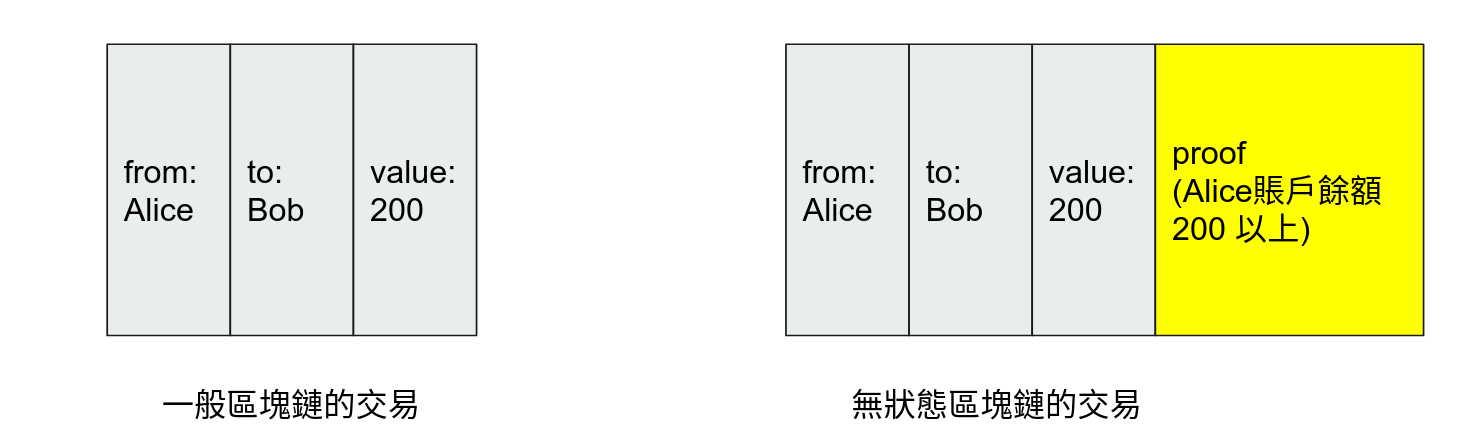
\includegraphics[width=\textwidth]{stateless-tx}
\caption{一般區塊鏈、無狀態區塊鏈交易比較}
\end{figure}

\subsection{vector commitment}

不僅僅上述的梅克爾樹變形能夠生成、更新摘要和證明,
可以做到這些功能的結構被稱為 vector commitment\cite{catalano2013vector}。

近年來, vector commitment 領域也持續出現不同針對無狀態區塊鏈的代數構造,
它們相較於梅克爾樹,時空間複雜度更小,或是擁有其他優點:
有的能夠將多個證明打包以降低空間\cite{boneh2019batching},
有的則有同態加法的特性,使得製作交易證明時,付款人不用知道收款人的當前餘額\cite{chepurnoy2018edrax}。

\section{快取證明}

Utreexo~\cite{dryja2019utreexo} 應用梅克爾樹構成的森林設計了一種新的 accumulator ~\cite{benaloh1993one},
基於此種 accumulator ,Utreexo 節點不需要真正的儲存比特幣所有的 UTXO ,
就能夠驗證區塊。

該篇論文也提及到,分析比特幣的歷史記錄,
約有 40\% 的 UTXO 會在 20 個區塊內被消耗,
將近 80\% 的 UTXO 會在 1000 個區塊內被消耗,
因此使用少量的記憶體空間來快取最近出現的 UTXO ,就能夠省略傳輸許多證明。

然而, Utreexo 僅僅討論了在初始同步節點資料時的情形,
並未考慮到同步到最長鏈之後可能發生的分叉問題。此外,
由於 UTXO 的產生與消耗都各只有一次,
使得具有統計性質的快取策略難以應用,而在賬戶系統中,
賬戶可以多次出現,因此可以應用的快取策略更廣泛。

本論文將會討論在賬戶系統中該如何應對分叉問題,
以及 LRU 快取策略在賬戶系統中的使用。

\subsection{持久化資料結構}

為了在分叉情況下高效存取快取,我們將會使用持久化資料結構,
故先行在此介紹基本概念與相關技巧。

如果一種資料結構在修改之後,能夠保留之前的版本,
就可以被稱為持久化資料結構\cite{driscoll1986making}(Persistent Data Structure),
與之相對的是暫時性資料結構(Ephemeral Data Structure)。

\subsubsection{路徑複製}
對於樹這種資料結構,可以利用路徑複製的技巧來將它變得持久化,
當樹中的一個節點被修改,就連帶修改指向它的父親節點,
如此一直遞迴往上修改到根節點,就可以得到一棵新版本的樹。

\begin{figure}
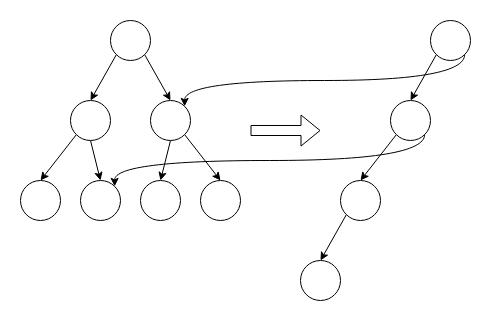
\includegraphics[width=\textwidth]{../images/路徑複製.png}
\caption{路徑複製}
\end{figure}

圖 2.2 是一個路徑複製的例子,可以從圖中看到,
只有被插入葉子的節點所在的分支被複製了一趟。

\graphicspath{ {./images/} }
\chapter{設計}
\label{c:design}

無狀態區塊鏈為了縮減硬碟佔用空間,必須在交易附上證明,導致所需網路流量增大;
為了省去硬碟隨機存取所耗用的時間,必須花費 CPU 計算能力來驗證證明。

無狀態區塊鏈相較於一般區塊鏈做出了一些取捨(trade-off),
而淺狀態區塊鏈的目的是讓這種取捨不再是全有或全無(全部都附上證明或全部不附上證明),
使得狀態儲存的程度變得可調節。

\section{淺狀態區塊鏈}

無狀態區塊鏈中的一個區塊,如果多份交易的付款人、收款人都相同,
交易的證明也會是完全相同的,這樣重複的資訊顯然可以省略。

擴展這個想法,如果我們快取最近出現過的交易中的賬戶資訊,
則下一次收到同樣賬戶的交易時,也不需要去驗證證明。

再更進一步,讓整個網路上的節點都遵循同一套規則來記錄快取,
使得所有節點對於什麼時候要附證明、什麼時候不用附證明有共識,
那在區塊廣播的時刻,節點就能夠剝離掉不必要的證明,進而省下網路流量。

淺狀態相對於無狀態,犧牲了一些記憶體空間,但是只要存取快取的速度快過驗證證明的速度,
淺狀態區塊鏈就有望在效能上勝過無狀態區塊鏈。

% TODO: 補以太坊交易的快取分析圖

如果節點在驗證同一個區塊時,使用的快取不一致,
將會導致某些節點承認該區塊,某些節點不承認,從而導致分叉。

譬如,如果節點快取住它高度最高的 k 個區塊中的交易資訊,
當網路延遲,不同節點中的鏈分叉情形不同時,快取就會不一致,見下圖:

\begin{figure}[h]
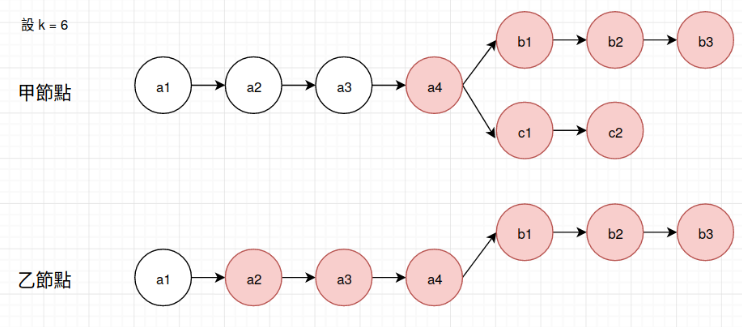
\includegraphics[width=\textwidth]{wrong-cache}
\caption{不一致的快取}
\end{figure}

粉紅色表示在快取,白色區塊則表示不在快取。
此時若有一個不附證明的交易,付款方在 a2 區塊出現過,則乙節點會接收交易,甲節點則不會接收。

\section{快取設計}

一個簡單的設計準則可以避免前述的錯誤:每一個區塊都有自己的快取,
快取的內容僅僅由該區塊所在的鏈的資料所決定。如此,我們把樹狀結構縮減為一個串列(list),
而不同節點上同個區塊所在的串列必定是相同的,只要每個節點都用同樣的確定性算法從這個串列計算出快取,
就能夠保證每個節點驗證同一個區塊時的快取一致。

\subsection{分叉處理}

觀察以下這條鏈:

\begin{figure}[h!]
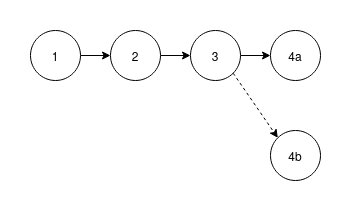
\includegraphics[width=10cm]{快取分叉}
\caption{區塊鏈分叉}
\end{figure}

此時,區塊 4b 嘗試接上區塊 3 ,因此它必須基於區塊 3 的快取來進行驗證。
也就是說,如果我們在接上區塊 4a 時,將區塊 3 的快取直接修改而稱為區塊 4a 的快取,
那當我們要街區塊 4b 時,就無從知悉區塊 3 的快取了,使用某些快取策略時,
我們可以透過回退(roll back)來取回區塊 3 的快取,但當使用某些快取策略時,遺失的快取無法輕易找回。

即使使用可以回退的快取策略,當分支切換越頻繁,回退的次數也會越頻繁,
而回退的效能可能就會成為瓶頸。

例如在圖 3.3 中,如果同時維持 a, b 兩條分支,則每次接收到非當前分叉的區塊時,都要進行回退,
並且隨著分叉的差異越大,回退的長度也越長,若從 7a 要走到 7b ,就必須先退回 3 ,再走回 7b ,
若之前曾經從 6a 走到過 6b ,則過程中的大部分運算都是相同的,這顯然是一種浪費。

\begin{figure}[h!]
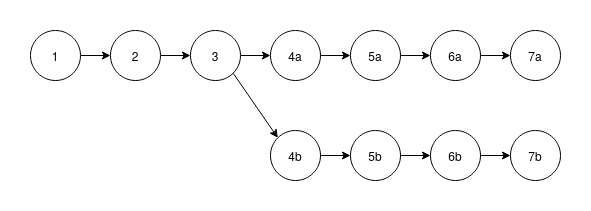
\includegraphics[width=\textwidth]{快取長分叉}
\caption{分叉頻繁切換}
\end{figure}

\subsection{持久化快取}

我們採用另外一種思路:在每個區塊上都保留它自己的快取,當新區塊要接上鏈的時候,
就可以直接取用它前一個區塊的快取,無需重新計算。
換句話說,我們採用全持久化資料結構(fully persistent data structure)~\cite{driscoll1986making}來儲存快取,
每接受一個區塊,就生成一個快取的版本。

在這個方案中,我們必須定時刪除太舊(例如,距離最長鏈超過 20 個區塊)區塊的快取,
以將整條鏈的快取大小限制在一定範圍,否則任由快取無限增長,將導致記憶體用罄,
以致於必須使用到硬碟,快取就變得沒有意義了。

這個方案帶來了一個立即問題,如果我們每次都複製前一個區塊的快取,
那快取的所佔用的空間將會正比於未刪除的快取的數量。
然而,相鄰區塊中的快取有很高的相似性,若能選用適當的資料結構來讓相鄰區塊共享快取,
將能夠有效提高空間使用率。

\section{快取策略}

不同的快取策略在應對不同工作量(workload)時的命中率(hit rate)各不相同,
以下討論實作簡單的「最近 k 塊」策略、FIFO 策略,以及實作較為複雜,但經驗上命中率較高的 LRU 策略。

\subsection{最近 k 塊}

在「最近 k 塊」策略中,一個區塊的快取即為由該區塊開始,由高往低取 k 個區塊,
這 k 個區塊中出現過的交易中的資訊。

以下為 k = 6 的示意圖

\begin{figure}[h]
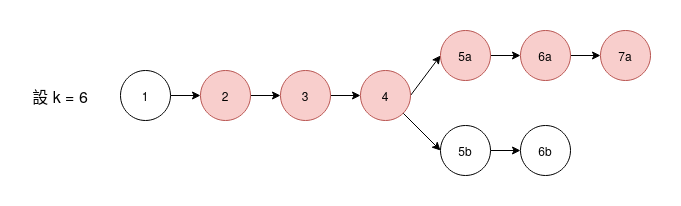
\includegraphics[width=\textwidth]{最近k塊}
\caption{區塊 7a 為粉紅色區塊中的所有交易資訊}
\end{figure}

可以用一個鍵值對(key value pairs)(其底層可為雜湊表(hash table)、平衡搜尋樹(balenced search tree)、跳錶(skip list)......等等)來表示快取,
若考慮每次重算的情境,例如在圖 3.4 中,要在 7a 後方額外加入一個 8a 區塊,
則我們加入 8a 區塊中的交易資訊,並丟掉只在 6a 中出現但沒有在其餘區塊中出現的交易資訊。

「最近 k 塊」的快取可以回退,跟前進時的算法一樣,只是換了個方向。

當考慮全持久化時,我們可以選用可持久化的鍵值對資料結構,
例如雜湊\cite{bagwell2001ideal}\cite{puente2017persistence}、搜尋樹都有相對應高效成熟的持久化實作,
若一個快取有 n 個鍵,則持久化雜湊/搜尋樹插入/刪除一筆鍵值時,
時間、空間複雜度皆為 $O(log(n))$。

\subsection{LRU}

LRU 是 least recently used 的縮寫,這種策略中,快取大小是固定的,
若快取已滿,在插入新資料之前必須先丟棄一筆資料,
LRU 會去挑選快取中所有資料中最久沒被用到的那一筆來丟棄。

LRU 之所以比 FIFO 的命中率更高,是因為以太坊的歷史數據顯示,
(1) 一個賬戶花錢之後,很可能又接著花錢。 (2) 一個賬戶收到錢之後,
很可能會馬上將錢花掉。LRU 由於會更新資料的使用時間,得以一直快取住頻繁出現的資料,
FIFO 則只看資料進入快取的時間,只要快取失效會發生,
快取需要被抽換,那即使某些資料頻繁出現,遲早還是會被丟掉。

抽象來看, LRU 是一種支援兩個介面的資料結構,

\begin{itemize}
  \item get(key)
  \item put(key, value)
\end{itemize}

get(key) 時,若 LRU 存在該鍵,則返回對應值,並且將 key 的使用時間調整到最新。

put(key, value) 時,若 LRU 空間未滿,直接插入一筆鍵值對,
這筆新鍵值對的的使用時間為最新;若 LRU 空間已滿,
就要找出當前快取中使用時間最舊的丟掉,再插入新鍵值對,此新鍵值對的使用時間亦為最新。

對應到淺狀態區塊鏈的情境中,每當一個區塊要接上,我們要計算新區塊快取時,
會把一系列帳號資訊的讀取跟修改操作轉變成 get 跟 put ,鍵是帳號地址,值是帳號狀態,
然後在 LRU 底層的資料結構上進行相應操作。

當在淺狀態區塊鏈中使用 LRU 策略時,是無法高效回退的。
插入一筆鍵值對時,要丟棄的資料可能在好幾個區塊之外,
然而被修改的 LRU 無從得知這筆資料要去哪個區塊尋回。

\section{持久化 LRU 算法}
在討論持久化 LRU 算法之前,我們先觀察如何在軟體上高效實作 LRU 快取,
調查 github 上多個高使用量的 LRU 函式庫,內部資料結構都是雜湊表與雙向鏈表(doubly linked list)的組合:

\begin{figure}[h]
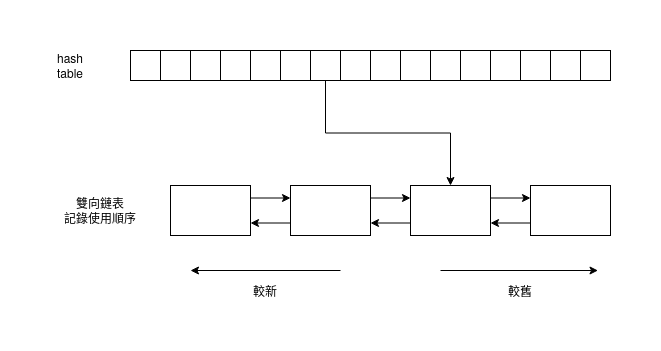
\includegraphics[width=\textwidth]{LRU}
\caption{LRU 資料結構}
\end{figure}

% TODO: 補圖

執行 get 時,透過雜湊得到指向節點的指針,獲取資料,並且將指針指向的鏈表節點移動至鏈表頭部(最左側)。
執行 put 時,若快取命中,更新節點的值,並將節點移動至鏈表頭部,
若快取未滿,從頭部加入快取值,並將其指針放入雜湊表,
若快取已滿,拔出雙向鏈表的尾部(最右側)節點,並且在雜湊表中移除該舊鍵,
然後在頭部加入快取值,放指針到雜湊表。

觀察到 LRU 需要記錄的資訊有二:

\begin{enumerate}
  \item 由鍵找到值(鍵值對)
  \item 各個鍵的順序資訊
\end{enumerate}

在前述的雜湊表 + 雙向鏈表的實現方案中,雜湊表負責 (1) ,雙向鏈表則負責 (2),
注意到,雙向鏈表極為自然的記錄了順序關係,它甚至不需要記錄確切的使用時間。

一個簡單的想法是,我們直接把雜湊跟雙向鏈表的持久化替代品組合起來,
就得到了一個持久化 LRU ,然而,雖然持久化雜湊有很成熟的替代品,
持久化雙向鏈表卻沒有。

因此,我們需要用其他可高效持久化的資料結構來取代雙向鏈表,進一步抽象雙向鍵表做的事情有:

\begin{itemize}
  \item 更新一個節點的使用時間到最新
  \item 刪除使用時間最舊的節點
  \item 插入新節點,新節點的使用時間為最新
\end{itemize}

以下,先討論了如何用紅黑樹\cite{guibas1978dichromatic}(平衡搜尋樹)來完成上述任務,
再介紹我們設計的順序樹資料結構,相比紅黑樹,它更加高效。

\subsection{雜湊 + 紅黑樹}

我們嘗試使用紅黑樹來記錄順序資訊。首先,為每一筆賬戶資訊設置一個獨一無二的時間序,
這個時間序可以很容易得到,例如說設置成 $block\_height * max\_tx\_in\_one\_block + tx\_number$。

然後,以時間序做為鍵,賬戶資訊為值,建造一棵紅黑樹。雜湊表則用賬戶地址為鍵,對應的時間序為值。

get 時,先在雜湊表中由賬戶地址得到時間序,再到紅黑樹中由時間序得到賬戶資訊。
例如,在圖 3.6 中,我們會先從雜湊表得到賬戶的時間序為 243 ,再到紅黑樹中查找 243 。

\begin{figure}[h!]
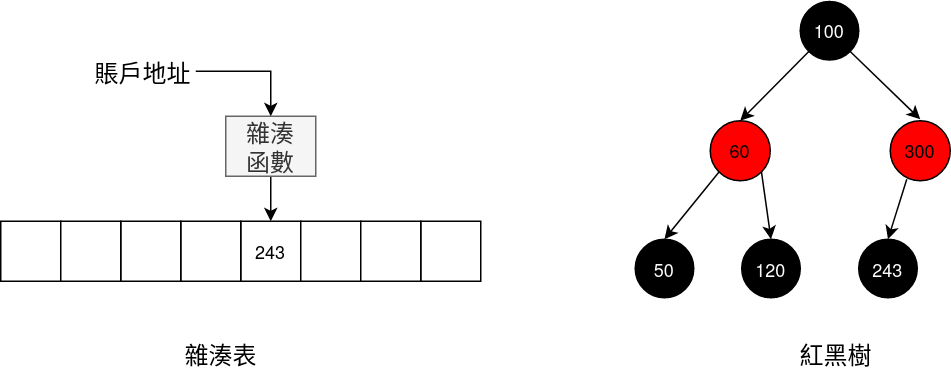
\includegraphics[width=\textwidth]{雜湊紅黑樹}
\caption{雜湊 + 紅黑樹}
\end{figure}

查找後,需更新使用時間。具體操作為修改雜湊表中地址對應的時間序,
並移除紅黑樹中的原節點,加入新時間序做為鍵。

put 類似於 get ,但需要修改賬戶資訊。

圖 3.6 表示不可變紅黑樹的共享結構。該圖中,快取的大小設為 8 。
狀態 1 時,只有 7 筆資料,狀態 2 對狀態 1 插入 14 ,資料變成 8 筆,
狀態 3 再對狀態 2 插入 15 ,由於快取已滿,必須先刪除時間序最小的資料,
也就是最左下角的紅色 7 。

\begin{figure}[h!]
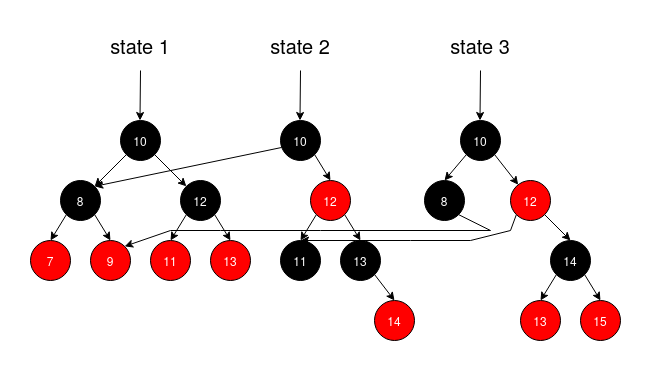
\includegraphics[width=\textwidth]{不可變紅黑樹}
\caption{不可變紅黑樹}
\end{figure}

% TODO:
% \subsubsection{紅黑樹 bulk 優化}

\subsection{雜湊 + 順序樹}

雙向鏈接串列以節點之間的指向關係記錄順序關係,紅黑樹卻必須額外記錄時間序,
此外,原本透過雜湊就能一次查找到賬戶資訊,紅黑樹方案卻得\emph{地址 -> 時間序 -> 賬戶資訊}兩段式地查找。

雙向鏈表無法以路徑複製來變換為不可變資料結構的原因在於,
兩個相鄰節點總是互指,一旦以路徑複製的方式修改節點,就得複製整個鏈表。
於是我們思考,不要用互指的方式來連接節點,就可以順利路徑複製。

想像在這些節點的背後編織一張網,然後將它們粘在一起(圖 3.8)。

\begin{figure}[h!]
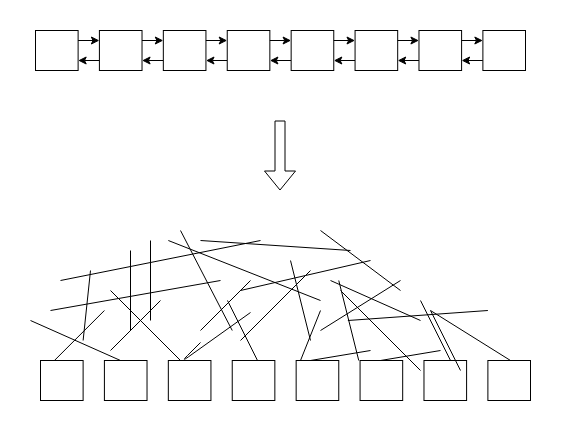
\includegraphics[width=\textwidth]{節點網}
\caption{}
\end{figure}

這個網狀結構最簡單形式就是一棵滿二元樹(full binary tree)(圖 3.9)。

\begin{figure}[h!]
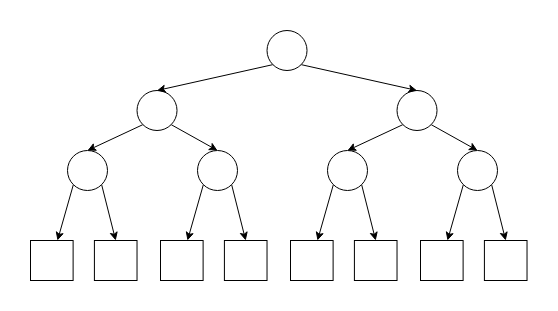
\includegraphics[width=\textwidth]{滿二元樹}
\caption{滿二元樹連接節點}
\end{figure}

我們將利用滿二元樹來儲存順序資訊的資料結構稱為順序樹,
以下開始一一介紹順序樹的各種操作。

若快取的容量為 $n$ ,順序樹的高度將會設置為 $1 + \lceil \log_2 n \rceil$,
也就是說,葉子的數量至少是快取容量的兩倍。圖 3.10 就是一棵容量為 4 的順序樹,它有 8 個葉子節點。

\begin{figure}[h!]
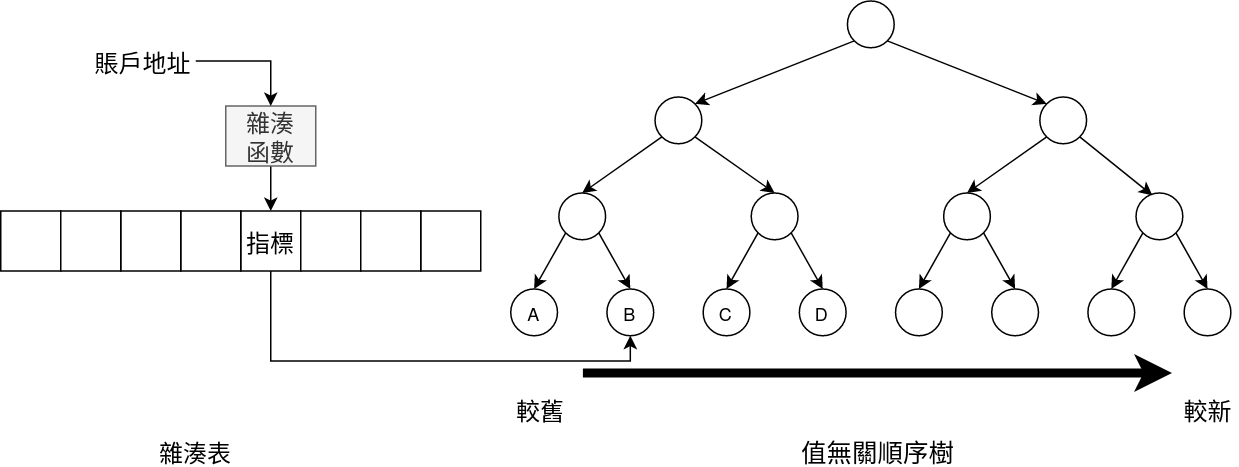
\includegraphics[width=\textwidth]{雜湊順序樹}
\caption{雜湊 + 順序樹}
\end{figure}

應用於 LRU 快取時,雜湊表所儲存的值會是一個指向順序樹葉子節點的指針,
只要一次雜湊表查詢就能取得資料。(見圖 3.10)

順序樹將所有資料都存放在葉子節點,每份資料按照使用時間的新舊來排列,
本文往後都按照資料越新,葉子的位置越右側的慣例來解釋跟畫圖。

順序樹的葉子有些有存放資料,有些沒有,我們將有存放資料的葉子稱為「有用葉子(used leaf)」,
沒有存放資料的葉子稱為「無用葉子(unused leaf)」。

get 時,將被查詢到的有用葉子改為無用的,並在當前最右有用葉子再往右一個的無用葉子中寫入原葉子的資料。
put 時,先找出最左側的有用葉子,將之改為無用的,並且在當前最右有用葉子再往右一個的無用葉子中寫入資料。

無論是 get 還是 put ,每次都會往右多佔用一個葉子,
如果當前最右的有用葉子已經在整棵樹的最右側了,就必須執行一次全複製,
把所有有用的葉子節點按照原本的順序緊密的排列在新順序樹的左側。

圖 3.11 演示了一連串的順序樹操作,其中狀態 7 到狀態 8 的時候發生了全複製。
圖中淺藍色節點表示它是無用的,注意到我們將所有葉子都無用的子樹的所有節點也都塗成淺藍了。

\begin{figure}[h!]
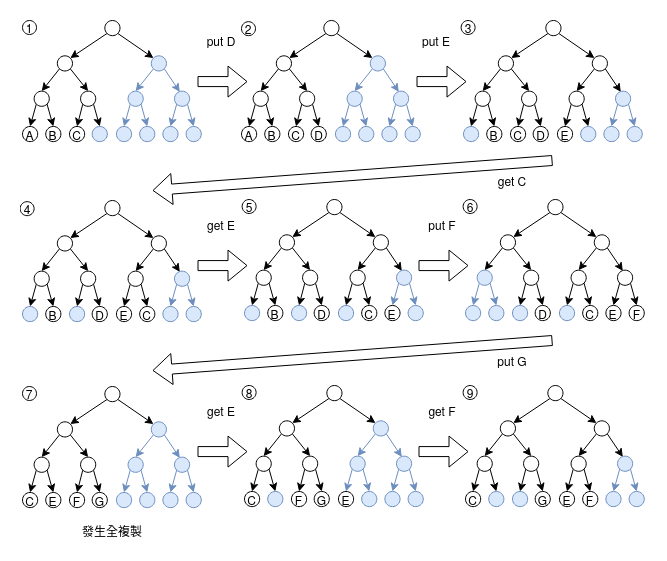
\includegraphics[width=\textwidth]{順序樹連續變化}
\caption{對順序樹進行一連串操作}
\end{figure}

在實作中,不需要真的為淺藍色節點分配記憶體空間,指向純淺藍色子樹的指針會是一個空指針(null pointer)。

\subsubsection{操作細節}

我們再接著探討 get, put 的操作細節。

要如何找出最左側的有用葉子?
從根部開始往下,若左兒子非空,往左走,若左兒子為空,往右走,走到高度為零時,就走到最左側有用葉子了。

從雜湊表中得到有用葉子的指針時,要如何知道該葉子在順序樹中的位置,以刪除它?
在葉子節點中,會儲存一個序號表示自己是從左到右的第幾個葉子,刪除葉子時,會從根一路往下,
判斷 $index \& (1 << height)$ 是否為 0 來決定往左還是右。

\subsubsection{時空間複雜度分析}

以下分析中,順序樹容量皆為 $n$ 。

若沒有發生全複製,get, put 都從根到葉子兩次,順序樹的高度是 $O(\log n)$,
時空間複雜度都是 $O(\log n)$。

如果發生全複製,就得遍歷一次順序樹,將所有有用葉子集結建一棵新樹,
注意到滿二元樹的總節點數量是葉子數量 * 2 - 1,不會超過 $n * 4$ ,
因此全複製的時空間複雜度是 $O(n)$ 。

$O(n)$ 的複雜度似乎有點高,但是每一次的 get/put 操作都只會讓有用葉子往右走一格,
至少要 n 次操作,才會使有用葉子走到整棵樹的最右側,
因此,若把全複製的成本攤銷到每一次操作,時空間複雜度是 $O(1)$ ,
get, put 的時空間複雜度依然是 $O(\log n)$ 。

嚴格來說,一個葉子的佔用的空間是 $O(\log n)$ ,因為葉子必須記錄自己的序號,
而序號在二進位的長度與順序樹的高度相同。但這不影響前述的空間複雜度分析,
即使考慮這點,時空間複雜度依然是 $O(\log n)$ 。
況且,實作中不可能會創建容量超過 CPU 位址空間大小的順序樹,
序號必定能用 64bit 的整數存下。
\chapter{實驗設計與結果}
\label{c:experiment}

在本章中,我們將在不同工作量下評估
以不同資料結構分別實作的持久化 LRU 性能。

\section{實驗環境}
實驗均在以下環境中進行

\begin{itemize}
\item CPU: AMD Ryzen 7 2700X (8 核心 16 執行緒、3.6 GHz、32K L1d 快取、64k L1i 快取、512K L2 快取、8M L3 快取)
\item 記憶體: DDR4 64 GB
\item 作業系統:Linux manjaro 4.19.36-1-MANJARO x86\_64
\item 編譯器: GCC 9.1.0
\end{itemize}

\section{資料結構}

我們以 C++ 17 撰寫了三種資料結構:

除了 3.4.1 節提到的持久化雜湊 + 持久化紅黑樹,
以及 3.4.2 節提到的持久化雜湊 + 持久化值無關順序樹之外,
還實作了雜湊 + 雙向鏈表的資料結構,
這是最簡易的持久化 LRU 實作,
它的各項操作與我們在 3.4 節介紹的暫時性 LRU 資料結構相同,
但當它需要創建新版本時,
會複製一份舊版本再繼續操作,
我們以此來對照具有共享結構特性的其他兩個持久化資料結構。

\begin{itemize}
\item 雜湊 + 雙向鏈表(3.4 節)
\item 持久化雜湊 + 持久化紅黑樹(3.4.1 節)
\item 持久化雜湊 + 持久化值無關順序樹(3.4.2 節)
\end{itemize}

由於要模擬的是區塊鏈,所以所有的工作量都以區塊為單位,
而一個區塊會包含多個 get/put 。
為此,以上三種的持久化資料結構的實作都支援了 transient \cite{puente2017persistence},
也就是說,資料結構不需要對每一個 get/put 都生成一個新版本,而是暫時生成一個版本,
在其上進行多個操作,再將它固定為不可變的,
由於減少了大量的中間狀態,此舉能夠大幅提升效能。

函式庫使用方面,雜湊直接使用了 C++ 標準函式庫的 unordered\_map ,
持久化雜湊則採用了著名的 C++ 不可變資料結構函式庫 \href{https://sinusoid.es/immer/}{immer} ,
其餘的雙向鏈表、持久化紅黑樹、持久化值無關順序樹則自行撰寫。

往後,我們會以雙向鏈表、紅黑樹、值無關順序樹來簡稱這三個複合資料結構。

\section{速度}

\subsection{工作量}
我們採用一個簡單的模型來模擬區塊生成,網路中有 n 個節點,
每個節點都會針對自己認定的最高區塊(亦即,它所認同的最長鏈的頂端)挖礦,初始時,
每個節點的最高區塊都是創世區塊(genesis block)。其後,有若干回合,
每個回合中,每個節點有一定概率會挖出新區塊。若它沒有挖到,
則會投奔其他節點挖出的同最高區塊的後繼區塊,若該最高區塊沒有任何後繼區塊,
則會隨機投奔其他最長鏈。若沒有任何節點挖到礦,就將同樣的過程再來一次。

在所有的工作量中,都是假定網路中有 10 個節點、每個節點在一個回合內挖到礦的機率是十分之一,
並且在挖出 1000 個區塊之後停止。在此設定下,同個高度大約會有 1.5 個區塊。

從 \href{https://etherscan.io/chart/gaslimit}{etherscan} 可以得知,
以太坊現今的 gas limit 大約是一千萬,而一筆交易的 gas 費用為 21000 ,
一個區塊大約可以包含 500 左右的交易。因此工作量的一個區塊的 get/put 指令數量設定為 500 。

此外,還有一項參數是 get/put 的佔比,對於一般的以太坊交易而言,
每次的付款都會導致賬戶的狀態改變,然而智慧合約的情形就不一定,
因此 get, put 兩種指令都有可能出現,以下若無額外說明,put 都占 50\% (get 也占 50\%)。

在開始任何一項工作前,我們都會先將整份快取裝滿,若非如此,當快取大小設定太大時,
需要很長一段時間才能將它裝滿,快取未滿時的狀態並非我們關注的,因為區塊鏈動輒幾百萬個區塊,
極大部分時間,快取都是裝滿的。

\subsection{調整快取大小}

第一項實驗將快取命中率固定在 100\% ,調節快取的大小(鍵值對的數量)。

\begin{figure}[h!]
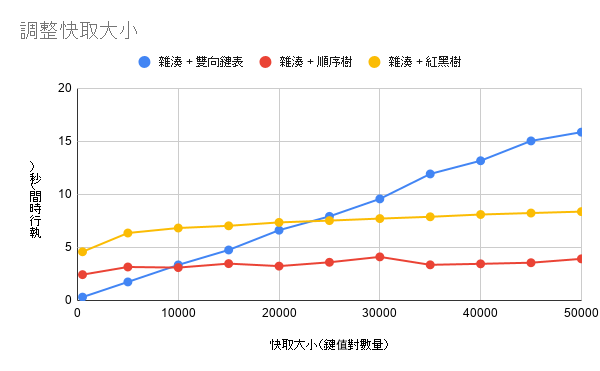
\includegraphics[width=\textwidth]{調整快取大小}
\caption{調整快取大小}
\end{figure}

所畫出的折線圖 4.1,可以看出,雙向鏈表所耗費的時間基本上正比於快取的大小,
顯見雙向鏈表的主要消耗在於複製,快取有多大,每次區塊更新,所要複製的量就有多大。

紅黑樹和值無關順序樹的成長曲線就十分平緩($O(\log n)$),而值無關順序樹的常數又小於紅黑樹。
注意到值無關順序樹的折線中,相較紅黑樹的穩定增長,是有所震盪的,
這跟值無關順序樹的葉子數量是 $1 + \lceil \log_2 n \rceil$ 有關,它的葉子數量更加離散,
當快取大小達到 $2^k$ 次方時,葉子數量往上翻倍,此時就會影響效能,導致震盪。

\subsection{調整快取命中率}

將快取大小定為 30000 ,調整命中率 。

\begin{figure}[h!]
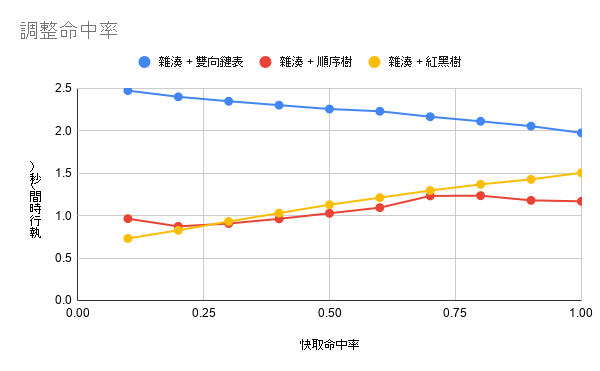
\includegraphics[width=\textwidth]{調整命中率}
\caption{調整命中率}
\end{figure}

圖 4.2 中可見,命中率對雙向鏈表並沒有什麼影響,因為它的主要消耗來自於複製,
快取命中之後要做的事情只是搬動幾個指標,不花什麼時間。
而紅黑樹、值無關順序樹的耗時都會隨命中率提高而有所上升,
因為它們主要的耗時來自於路徑複製,命中越多,需要複製、創建的分支也就越多。

\subsection{調整 put 比例}

將快取大小定為 30000 ,命中率設為 1.0 ,調整 put 佔兩種指令的比例。從圖 4.3 可見基本不影響效能。

\begin{figure}[h!]
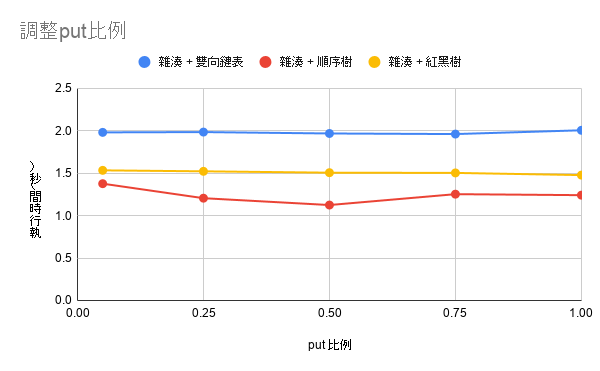
\includegraphics[width=\textwidth]{調整put比例}
\caption{調整 put 比例}
\end{figure}

% \subsection{記憶體用量}

\section{失效代價(miss penalty)}

如果驗證一筆交易時,它相關賬戶的資訊不在節點的快取中(快取失效),
這筆交易就得附上證明以供節點驗證。因此快取失效的代價有二:
(1) 接收證明所需要的網路 I/O ,這與證明所佔的空間有直接關係。
(2) 驗證證明所消耗的 CPU 運算時間。

而快取命中所耗費的時間,我們可以觀察圖 4.3 ,
值無關順序樹實作在快取大小 30000 、put 比例 100\%、命中率 1.0 時,
 1.241 秒內執行了 1000 個區塊,而一個區塊中有 500 條指令,
亦即一個區塊的平均執行時間是 1.241 毫秒,當快取更小的時候,這個數字還會更低。

我們挑選最常見的梅克爾 Patricia 樹的驗證成本來與值無關順序樹實作比較,
函式庫選用了兩大以太坊實作之一的 \href{https://www.parity.io/ethereum/}{Parity Ethereum}
的 \href{https://docs.rs/trie-db/0.20.1/trie_db/index.html}{trie-db} 模組。

影響梅克爾 Patricia 證明的因素有二:
(1) 葉子的數量 $s$ ,證明的大小就約為 $O(\log s)$ , 要驗證一個證明的時間複雜度也是 $O(\log s)$ 。
(2) 批量處理時,一批的數量。梅克爾證明就是梅克爾樹的一個分支,當一個節點被多個分支共享時,不必重複計算,
因此一次驗證 $k$ 個證明的時間會短於 $k$ 乘以驗證一個證明的時間。

由 \href{https://www.etherchain.org/charts/totalAccounts}{etherchain.org} 的資料我們可以得知,
現今的以太坊賬戶數量已經超過八千萬,
所以我們先在梅克爾 Patricia 樹中隨機插入八千萬筆資料(也就是說葉子的數量為八千萬),
並且根據此前一個區塊中 500 個交易的假設,批量驗證 500 個證明,
量測得到所費時間 5.536 毫秒,明顯要比直接取用快取來得耗時。

而一個區塊的證明大小約為 900 KB ,1000 個區塊就是將近 900 MB ,
若使用當今一般的家用網路,下載這些額外證明所需的時間又比驗證證明更加耗時。

\section{總結}

實驗驗證了值無關順序樹、紅黑樹較低的時空間複雜度,在快取大小增大到一定程度後,
表現上顯著領先總是複製自身的雙向鏈表。 而值無關順序樹相較於紅黑樹,
在效能上並無顯著優勢,但其在概念上易於理解\footnote{此爲作者的主觀認知}(無各種旋轉規則需記誦),
時間複雜度相當,若未來有人想於無狀態區塊鏈上實作 LRU 快取,
亦可考慮使用值無關順序樹。

同時也實驗、量測了梅克爾 Patricia 樹的證明大小以及驗證速度,
瞭解到通常情況下直接讀取快取要比下載、驗證證明要來得快速。
根據這些數據,能夠推論若以梅克爾 Patricia 樹做為 vector commitment 時,
淺狀態區塊鏈若採取適當的快取大小,能夠在 LRU 策略下帶來速度提升。
% \chapter{相關研究}
\label{c:related}

\section{Utreexo}
Utreexo~\cite{dryja2019utreexo} 應用梅克爾樹構成的森林設計了一種新的 accumulator ,
基於此種 accumulator ,Utreexo 節點不需要真正的儲存比特幣所有的 UTXO ,
就能夠驗證區塊。

然而,比特幣網路已經存在多年,大幅修改協議使得所有節點改為無狀態並不現實,
Utreexo 提議可以採用一個橋接節點作為比特幣全節點與 Utreexo 節點的中介,
當區塊廣播由 Utreexo 節點到全節點時,會剝離掉證明,反之則補上證明。

該篇論文也提及到,分析比特幣的歷史記錄,
約有 40\% 的 UTXO 會在 20 個區塊內被消耗,
將近 80\% 的 UTXO 會在 1000 個區塊內被消耗,
因此使用少量的記憶體空間來快取最近出現的 UTXO ,就能夠省略傳輸許多證明。

與本研究的差別在於,本研究考慮基於帳號的虛擬貨幣,而非基於 UTXO 的,
同時,本研究也額外考量了分叉時的情況。

\section{Making Data Structure Persistent}
該篇論文~\cite{driscoll1986making}提出了多種算法能夠使得任何基於節點的資料結構半/全持久化(partial/fully persistent),
根據該論文的 node-splitting 算法,
甚至能夠在 $O(1)$ 時間複雜度內完成雙向鏈表的插入、修改。

然而,該論文並沒有提出刪除持久化資料結構的過去版本的方法,
這使得這些算法難以應用到淺狀態區塊鏈的快取上,
因為無法刪除過去版本將導致快取所需的空間始終無法釋放,
最終耗盡記憶體容量。
\chapter{未來工作}
\label{c:future_work}

\section{更多快取策略}
工作量(workload)不同時,最佳的快取策略也不同,
FIFO, LFU, Second-chance, .... 等等快取策略若要應用進淺狀態區塊鏈,
就必須分別設計如何持久化地儲存它們。

\section{快取拆分}

若要讓淺狀態區塊鏈支援智慧合約,單以一個賬戶為快取單位會導致一些問題,
因為每個智慧合約的狀態所佔用的空間可能相差巨大,如果快取中的每一個狀態都非常大,
那整個快取就會佔用很多空間,反之若快取中的狀態都很小,整個快取佔用空間就很小,
當快取佔用的空間不穩定時,節點的維護者就很難為自己的機器設定參數。

我們可以借鑑作業系統的分頁設計,將智慧合約的狀態切割成等體積的多個小塊,
每次快取只會存取到用到的小塊,如此就能夠使快取佔用空間變得穩定。

% \section{隨機化順序樹}
% TODO
%\input{photoshoot}
%\input{modeling}
%\input{application}
\chapter{總結}

本論文描述了淺狀態區塊鏈的設計,
並探討了多種快取策略的優缺點。特別對於 LRU 快取策略,
我們先嘗試持久化雜湊加持久化紅黑樹的組合,
再提出了一種新穎的資料結構,值無關順序樹,讓它與持久化雜湊組合,
得到一種複雜度相當的持久化 LRU 實作,
最後,討論了基於持有化雜湊搭配持久化堆積的 LRU 實作,
它的複雜度也與上兩者相當。

\appendix

\backmatter

\addcontentsline{toc}{chapter}{\bibname}
\bibliographystyle{abbrv}

% Your bibliography goes here
\bibliography{thesis}

\end{document}
